\chapter{Service-oriented computing}
\label{chap:service-oriented computing}
\emph{Service-oriented computing} represents a distributed computing platform [1]. It has its own paradigm, logic, architecture and patterns. It is built on the distributed computing platforms and extends it by new considerations about governance, design layers and technologies suitable for its implementation.
\emph{Service orientation} is a design paradigm, it divides the system into logic units which are separately shaped and can be utilized according to strategic goals and benefits of a requested result.

\section{Service-oriented architecture}
\emph{Service-oriented architecture (SOA)} is a set of best practices for an organization leading to agile architectural model of the system to meet business needs. Result of applied practices is an architecture which corresponds to dynamic market changes. The SOA best practices are describing the human behaviour, there is no list of constraints which have to be followed to obtain a service-oriented architecture. The best practices are designed to resolve specific situations which the organization can meet and depending on them could be selected just a subset of appropriate practices which are necessary to apply.\par

The architecture is layered. Layers can be multiple and can differ according to needs of designed system. One of the examples of horizontal layers is designed in Figure \ref{fig:soa-architecture}. The layers are separated and each of them encapsulates its implementation so that another layer can't access and modify it (excluding potential harms). In this example provider develops an application containing services which have access to a database using adapter. The \textit{\gls{adapter}} serves to transform data from database to data useful for services and vice-versa. \textit{Services} are entry point for consumer application, thanks to them he has an access to the data without direct access to \textit{database}.

\begin{figure}[htp] \centering{
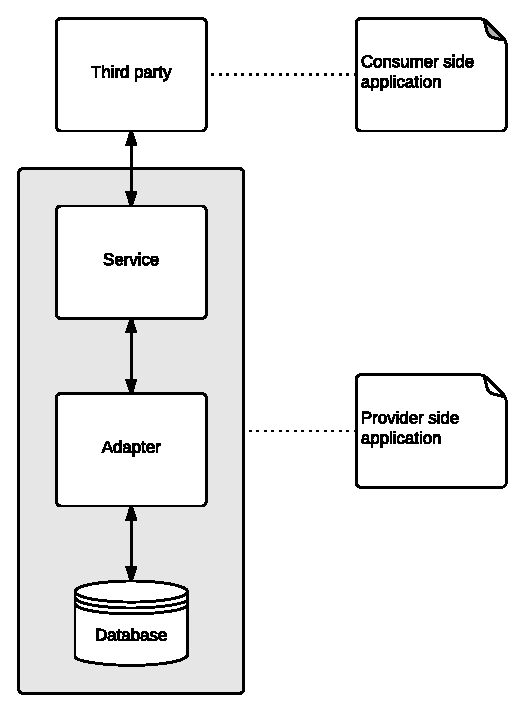
\includegraphics[width=8cm]{img/soa-architecture.pdf}}
\caption{Example of service-oriented architecture model}
\label{fig:soa-architecture}
\end{figure}  

One of the main advantages of a service-oriented architectural style is its ability to efficiently deal with changes. \textit{"SOA is based on a decomposition of enterprise IT assets and separation of 'stable' IT artifacts (services) from 'changeable' artifacts (business processes), orchestrating services into IT solutions (processes)."} \cite{website:versioning-in-soa}. %(http://msdn.microsoft.com/en-us/library/bb491124.aspx) 
Above mentioned services are essential part of SOA. Relationship between them and a business process constituted by services are visualized in the Figure \ref{fig:business-process-services}. The business process is a process from real world which workflow is simulated by services. A task of this process is composed by one or more of them. Services perform the logic, comunicate with underlied leyers to retrieve and store data to operate as a business process.

\begin{figure}[htp] \centering{
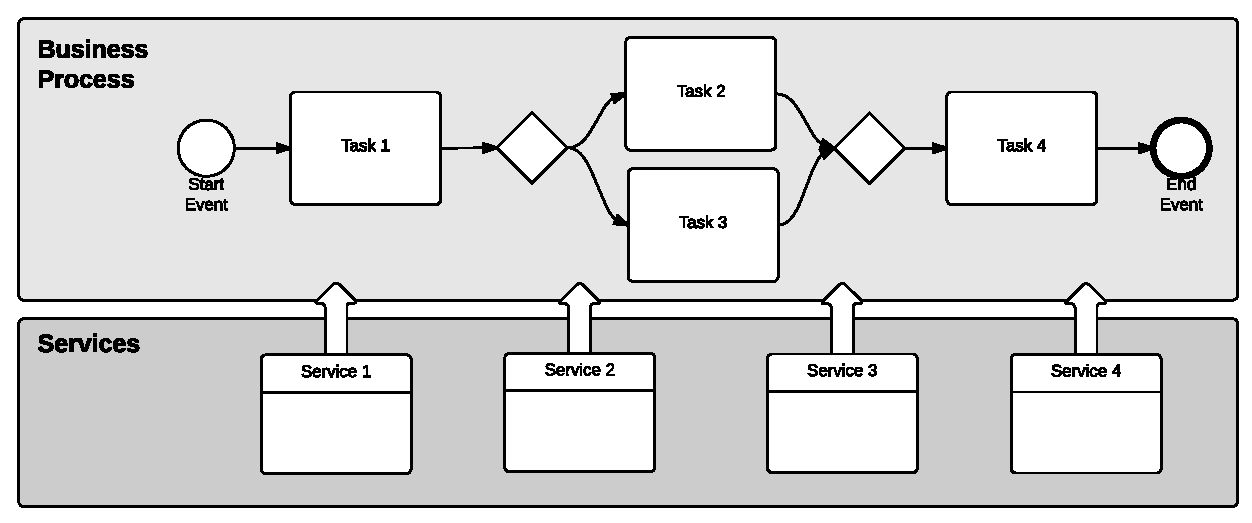
\includegraphics[width=12cm]{img/business-process-services.pdf}}
\caption{Business process is a composition of services}
\label{fig:business-process-services}
\end{figure} 

The speed of changes in the business department is too fast to be passed directly into development and maintenance of the monolithic systems. Functionality of these systems is designed on measure of customer and often can't deal easily with changes, it can arrive in interference in design of whole architecture. SOA offers better flexibility when business requirements change, changes are reflected into modification of an existing business process by changing involved services, or if it's needed a new process is created using existing services or a new service can be created. There are more approaches how to deal with the changes and one of them is versioning which is described in chapter \ref{chap:versioning} and \ref{chap:versionaccess} in detail.

\section{Services}
\label{sec:services}
Services are the logic units form which is composed the \gls{service-oriented-design}. Every service is standalone object or component. Every service has its own functional context and related capabilities. Each service is deployed independently on another one and on the system which use it. It allows a parallel development, one service can be a part of many products of the corporation.
\textit{"The essence of Service in the SOA context is the business abstraction - that is a representation of functionality and/or data presented in business context."} \cite{agile-architecture}

\subsection{Service lifecycle}
\label{subsec:lifecycle}
Services have their lifecycle, there are stages:
service-oriented analysis, service-oriented design, service logic design, service development, service testing, service deployment and monitoring, service usage and monitoring, service discovery, service versioning and retirement. \cite{soa-governance}

\begin{enumerate}
  \item Service-oriented ananlysis \\
  During this phase there are created the services candidates, their capabilities and compositions. The analysis is typically interative, for each business process is created a service inventory.
  \item Service-oriented design \\
  The stage designs the service contracts. For every service candidate it is considered a technical contract, in case of REST services (described in section \ref{sec:rest}) it is inevitable to think of HTTP method usage, resource identifiers and header parameters.
  \item Serivce Logic Design \\
  Phase establish the service architecture and its logic so that the service will carrying out the functionality resulted from the contract.
  \item Service Development \\
  The implementation of the services is performed. It is based on specifications and architecture design from previous stages.
  \item Service Testing \\
  The implemented services needs to be tested to provide the quality assurance of developed application.
  \item Service Deployment and Maintenance \\
  In this phase the services are deployed on production environment. Maintenance involves changes and upgrades of services regarding to production environment, but it doesn't include changes which would result in new version of services.
  \item Service Usage and Monitoring \\
  Deployed servise which is in use is an object of monitoring. It is essential for obtaining the numbers related to various metrics. Measured values can positively influence the maintenance and are further used for business assessment.
  \item Serivce Discovery \\
  Process of identifying \gls{agnostic-services} throughout the given service inventory.
  \item Service Versioning and Retirement \\
  After deployment and usage can arise a need for change of the logic of a service or addition of a new one. Emission of new serivce version occures. How to version the services will be explained accross the next sections. Retirement encompasses the termination of the use of the serivice. Regarding to service versioning a version of service which is no longer in use can be retired.
\end{enumerate}

\subsection{Levels of a service} 
\label{subsec:levels-of-service}

There are three levels of how we can interpret the expression \emph{Service} in SOA context \cite{agile-architecture}:
\begin{enumerate}
  \item \textbf{Service implementation} \hfill \\
Service implementation is the code performing the logic.
  \item \textbf{Service interface} \hfill \\ 
This level is an entry point to the service implementation, it provides underlying logic to consumers but encapsulating it in a way that consumers can see the implementation. 
  \item \textbf{Abstracted service} \hfill \\
Abstracted service or business service represents a business capability or data. This services can be composed to describe a business process. This is a core abstraction of SOA.
\end{enumerate}

There is a many-to-many relationship between these three levels. Business service can represents multiple interfaces and in the same time one interface can be supported by multiple implementation.

%TODO picture of service levels

%\subsection{Service categories and types} 

%There are two main types of services. The first type is composed by infrastructural services which provide the facilities and aren't a part of application. To the second type belongs services which are the part of the application and provide main logic.

\bigskip
%TODO describe services

%Service categories \cite{website:ontology-taxonomy} :
%\begin{description}
 % \item[Bus services] can be further divided into 
  %\begin{enumerate}
   % \item Communication services 
    %\item Utility services
  %\end{enumerate}
  %\item[Application services] consist of   
  %\begin{enumerate}
   % \item Entity services
    %\item Capability services
    %\item Activity services
    %\item Process services
  %\end{enumerate}
%\end{description}

%TODO image 

\section{Granularity}
\label{sec:granularity}
In SOA context granularity is often used expression, it is related to how much data is understood under one unit regarding to whole data pool. It is possible to distinguish between from fine-grained to coarse-grained granularity, where fine-grained contains small amount of data in one unit respective to whole data pool. On the contrary the coarser granularity bears much more data in one unit.

\subsection{Service granularity}
Service granularity is defined during analytical part of the service design. As it is written above services are composing the business processes.\par
Granularity determines properties of the services with respect to the processes. Services can be fine-grained up to coarse-grained. When services are fine-grained consequently the number of services is higher containing less logic therefore the costs for the implementation are smaller and the higher reusability is provided. However the effort needed to compose these services into a process is higher. 
On the other side when services are coarse-grained they contain more complex logic, are easily composing the process, but the reusability is limited and more effort is required to implement them.

\section{Approaches of implementation of web services}
Web services are one group of services, these are intended to work on a network such as the Internet.

\subsection{Evolution of approaches}
 
/TODO write shortly about RCP, WSDL, SOAP
%TODO form agile architecture revolution
 
\subsubsection{REST}
%TODO WADL ??

Representational State Transfer, REST is an architectural style for building distributed hypermedia applications. This thesis deals with REST architectural style and REST services. They will be described in detail within the next chapter. \ref{chap:rest}



%%\subsubsection*{\textbf{Guacamole} \hfill \emph{http://guac-dev.org/}}
%%\label{subsec:guacamole}
%% \ref{}.
%%    \item \textbf{[název předmětu 1]} \hfill \\
%%    odkaz na stránku předmětu, obsahující pouze název a informace o spolufinancování \gls{eu}
    
%%\begin{table}
%%  \caption{Základní typy entit v Drupalu}
  %%\label{tab:typy-entit}
  %%\begin{tabular}{ | p{3cm} | l | c | c | }
   %% \hline 
    %%Typ entity & Strojový název & Dostupnost polí & Rozšiřitelnost \\ \hline 
    %%Komentář & comment & \checkmark & \checkmark \\ \hline 
    %%Soubor & file &  & \\ \hline 
    %%Slovník & vocabulary &  & \\ \hline 
    %%Uzel & node & \checkmark & \checkmark \\ \hline 
    %%Uživatel & user & \checkmark & \checkmark \\ \hline 
    %%Záznam slovníku & term & \checkmark & \checkmark \\ \hline             
  %%\end{tabular}
%%\end{table}
%% \emph \emph \texttt.
